   
\documentclass[11pt]{article}
\usepackage{amsmath,amsthm,verbatim,amssymb,amsfonts,amscd, graphicx}
\usepackage{graphicx}
\usepackage{float}
\usepackage{url}
\graphicspath{{./times/}}
\topmargin0.0cm
\headheight0.0cm
\headsep0.0cm
\oddsidemargin0.0cm
\textheight23.0cm
\textwidth16.5cm
\footskip1.0cm

\begin{document}
\title{CS 5220\\ Project 1 - Matrix Multiplication}
\author{Sheroze Sheriffdeen(mss385)\\ Weici Hu(wh343)\\  Qinyu Wang(qw78)}
\maketitle

\section{Introduction}
\textbf{D}ouble Precision \textbf{GE}neral \textbf{M}atrix \textbf{M}ultiplication (DGEMM) is an important operation in problems in scientific and engineering computing applications. DGEMM takes 2 dense square double precision matrices $A$ and $B$ stored in column major format and returns,
	\begin{equation} 
		A \times B = C
	\end{equation}
	
	where '$\times$' represents matrix multiplication. This document describes an optimized DGEMM implementation and details the design decisions used to improve performance. 

\section{Implementation Overview}
\begin{figure}[H]
\centering
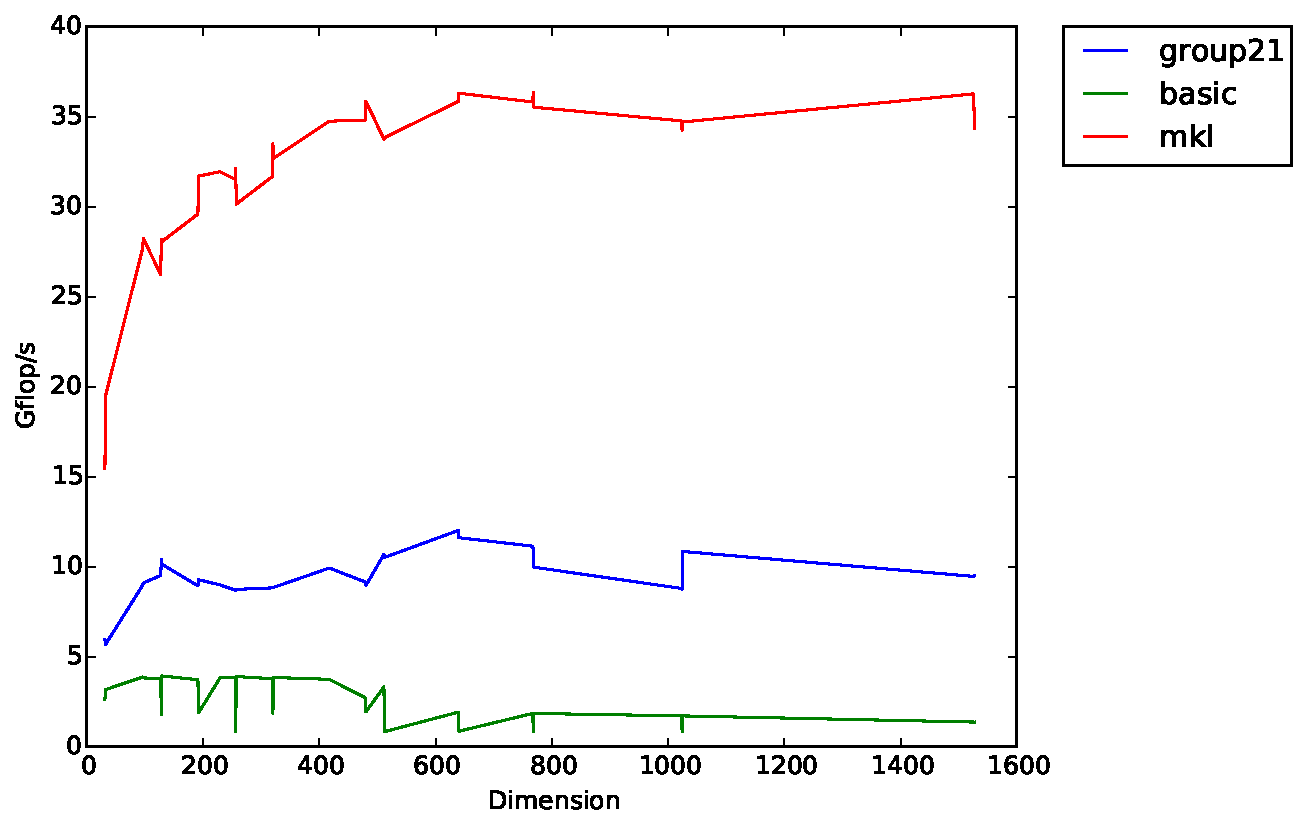
\includegraphics[scale=0.6]{growth_final.pdf}
\caption{Performance comparison: Intel MKL, our implementation and the naive implementation}
\end{figure}
\newpage
Our DGEMM implementation has 2 distinct modes of operation. On square matrices with leading dimension $<$ \texttt{BLOCK\_THRESHOLD}, our DGEMM uses tight loops with copy optimization. (Section \ref{sec:copy_opt}). \texttt{BLOCK\_THRESHOLD} was picked to be 1000 elements. The L2 cache of the  Intel Xeon E5-2620 v3 processor is 15MB and we are able to fit both $A$ and $B$ in the cache. \\

On matrices with the leading dimension $>$ \texttt{BLOCK\_THRESHOLD}, we switch to a blocked matrix multiplication. Each block has $32 \times 32$ elements. Prior to blocking, the matrices we perform copy optimization on $A$ and transpose and copy over data to a 64 byte aligned block obtained by Intel's \texttt{mm\_malloc}. Furthermore, we also copy over data from $B$ to an aligned block and create an aligned stored area for $C$. The newly allocation dynamic memory uses zero padding so that all block multiplication is similar. (Section \ref{sec:block}) \\

On each block, we perform the naive matrix multiplication using tight loops. To make use of the aligned data, we provide hints to the compiler by adding the $\texttt{\_\_assume\_aligned}$ clause prior to the loop using the matrix data. \cite{vectorization} Furthermore, since $A$ is transposed due to copy optimization, the innermost loop of the block multiplication is performed with stride 1. 



\newpage
\section{Design Decisions}
\subsection{Compiler Flags}\label{sec:comp_flags}
\subsection{Copy Optimization}\label{sec:copy_opt}
\subsection{Padded Blocking}\label{sec:block}
\subsection{Memory Alignment}\label{sec:align}

\newpage
\section{Steps that did not work}

\newpage
\section{Optimization Experiments}
\subsection{Block Multiplication with Multiple Block Sizes}
\subsubsection{Approach}
Working off of \texttt{dgemm\_blocked.c}, we tried different block sizes to examine the performance changes. 
\subsubsection{Results}
Figure \ref{pow_2_blocks} shows the performance of different approaches with various block sizes. (block sizes are a multiple of 2). The performance gain for varying block sizes is not immense but a block size of 64 performs better than other block sizes. \\

\begin{figure}[H]
    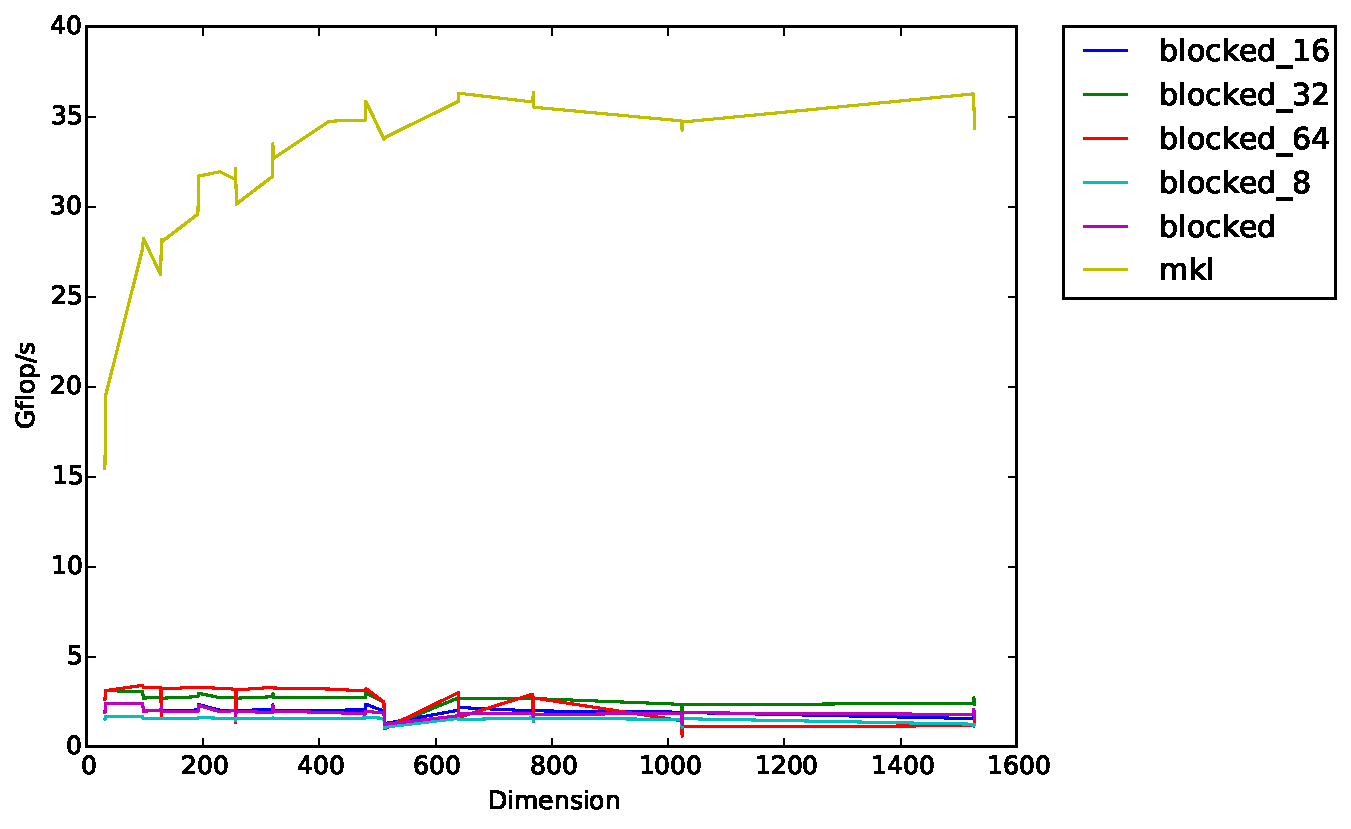
\includegraphics[width=0.9\textwidth]{timing_block_size_changes.pdf}
    \caption{Block size variation}
    \label{pow_2_blocks}
\end{figure} 

In addition, we attempted block sizes that are not a multiple of 2. Figure \ref{odd_blocks} is the comparison of the performance against a block size of 64.\\
\begin{figure}[H]
    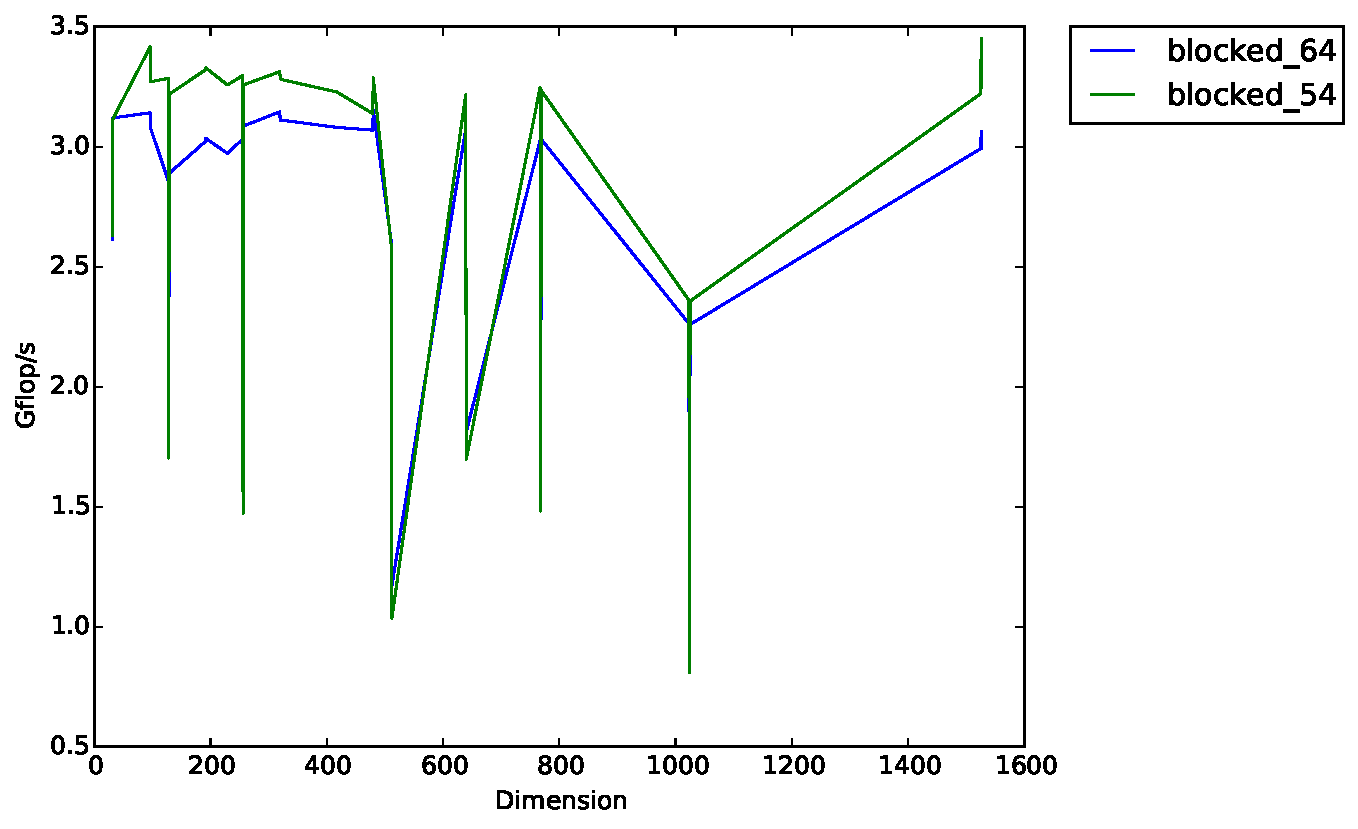
\includegraphics[width=0.9\textwidth]{timing_54_64.pdf}
    \caption{Block size variation}
    \label{odd_blocks}
\end{figure} 


\subsection{Block Multiplication with Manual Loop Unrolling}
\subsubsection{Approach}
In this approach, we manually unrolled 4 computations in the inner most loop of the matrix multiplication of a block. 
\subsubsection{Results}
Figure \ref{unrolled_vs_regular} compares the performance of the unrolled blocked version against the vanilla blocked approach. The unrolled versions clearly perform better than the original blocked approach but not by much. 
\begin{figure}[H]
    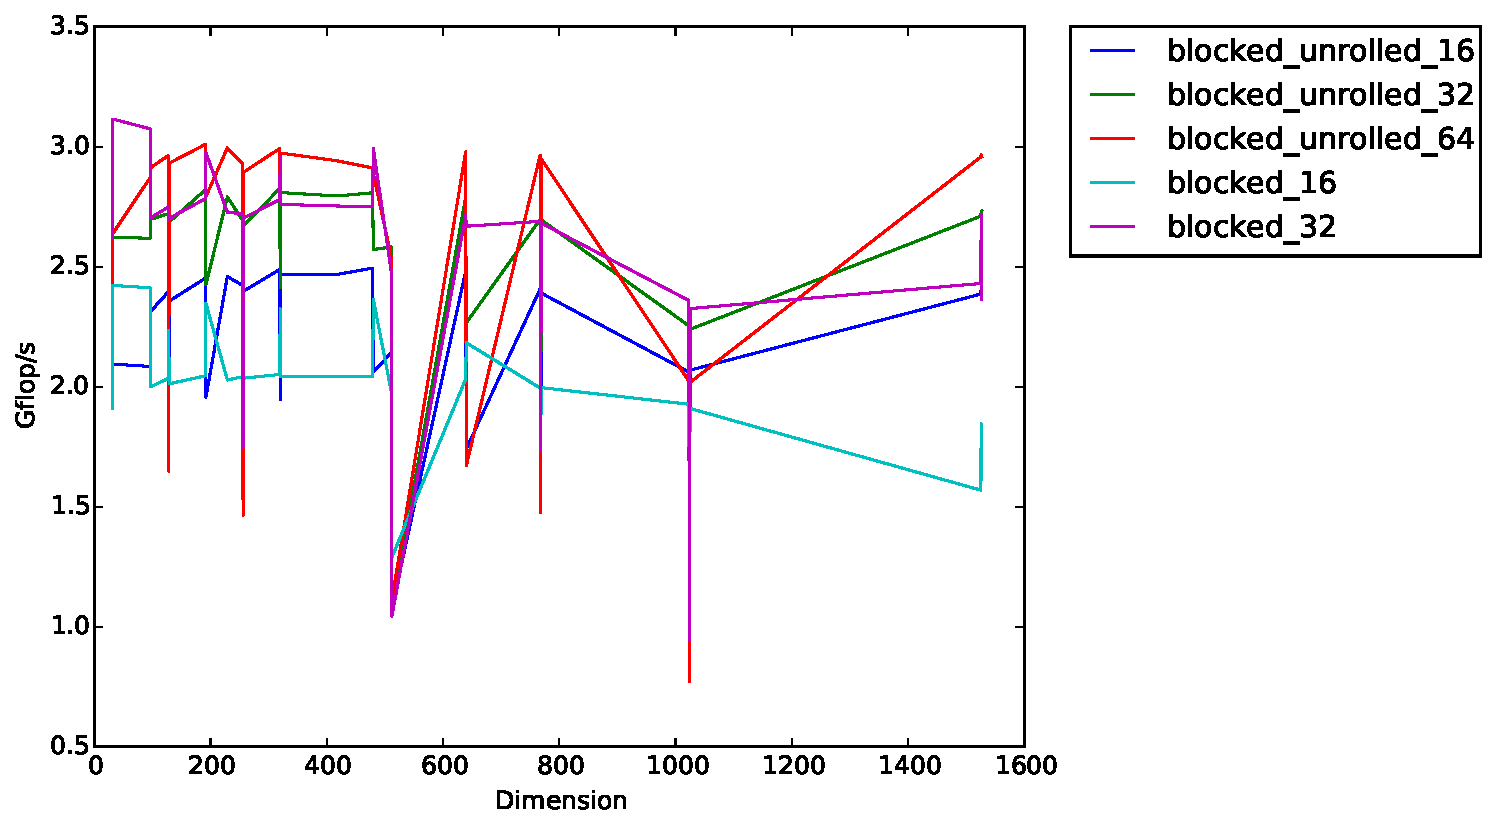
\includegraphics[width=0.9\textwidth]{timing_unrolled_vs_nonunrolled.pdf}
    \caption{Unrolled blocks vs regular blocks}
    \label{unrolled_vs_regular}
\end{figure} 

\subsection{Compiler Optimization Flags}
\subsubsection{Approach}
Using the blocked approach as a baseline, we examine the effect of various compiler flags on the multiplication.
\subsubsection{Results}
Figure \ref{all_optimized_blocked} shows the performance of blocked multiplication with the flags, \texttt{-O3 -march=native -funroll-loops}.
\begin{figure}[H]
    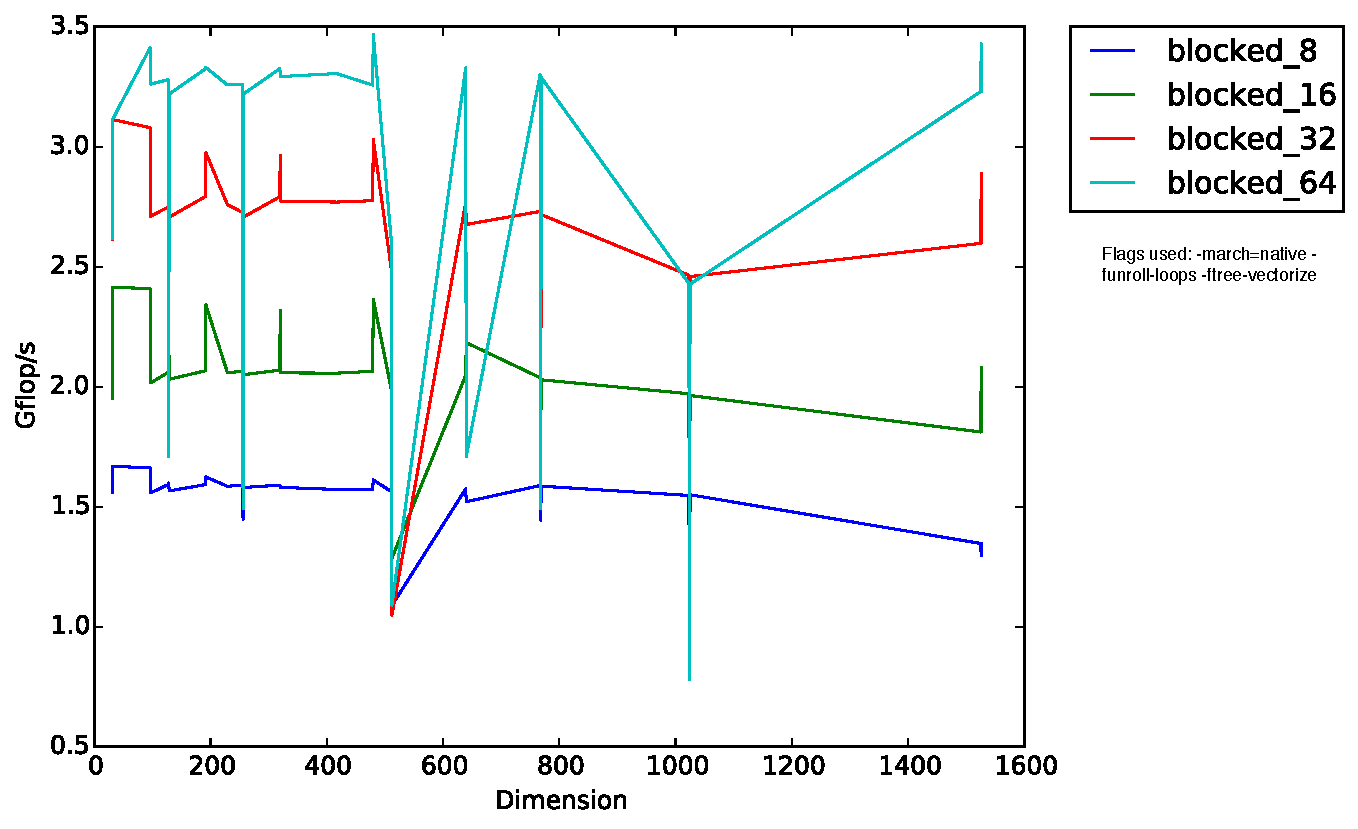
\includegraphics[width=0.9\textwidth]{timing_flags_blocked.pdf}
    \caption{Compiler flags \texttt{-O3 -march=native -funroll-loops}}
    \label{all_optimized_blocked}
\end{figure} 

Figure \ref{funroll_vanilla} shows the performance of blocked multiplication with the flags, \texttt{-O3 -funroll-loops} vs just \texttt{-O3}. It appears that merely having the \texttt{-O3} flag performs as well as having loops unrolled. 
\begin{figure}[H]
    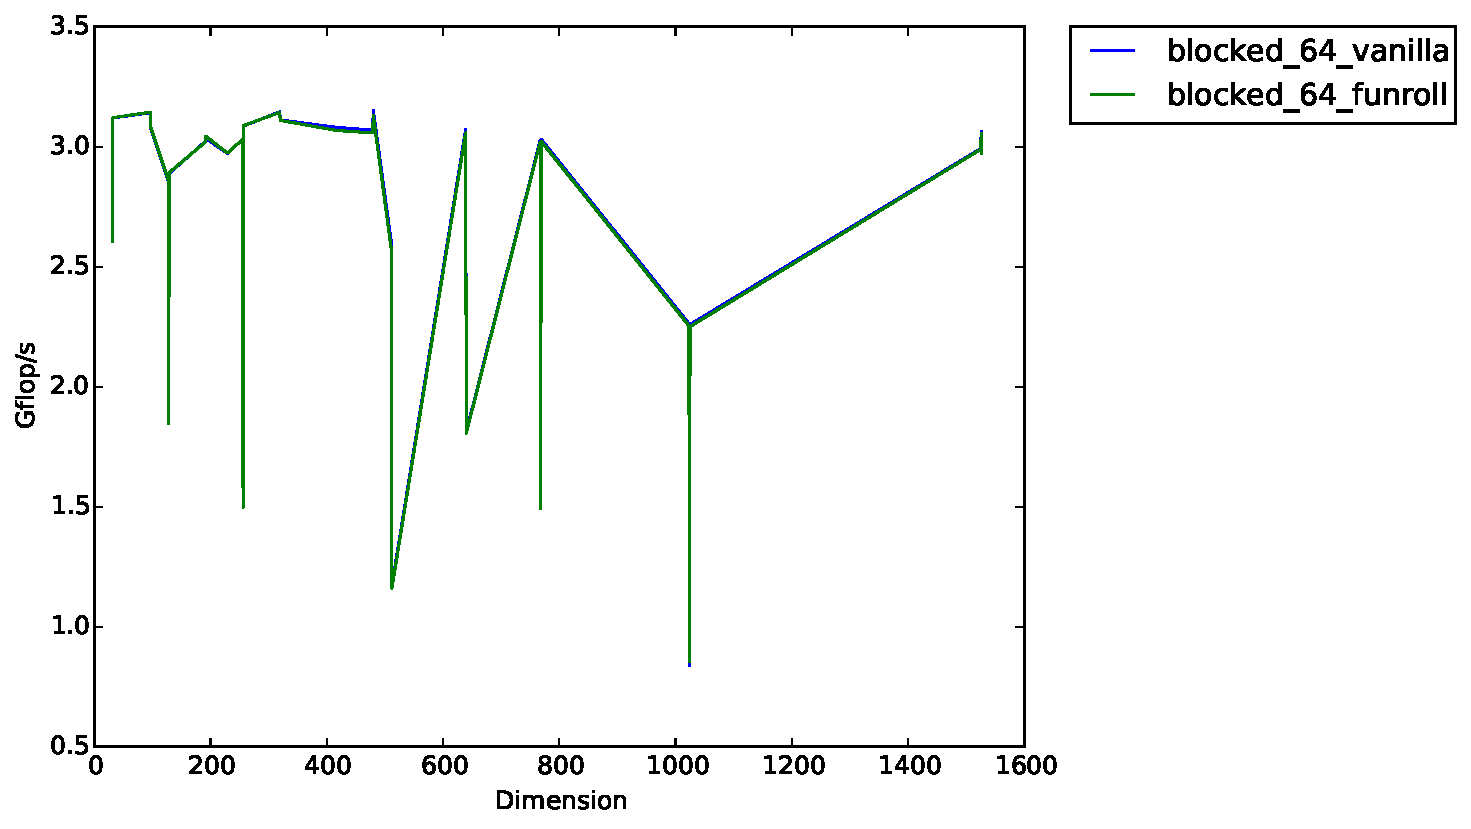
\includegraphics[width=0.9\textwidth]{timing_funroll_vanilla.pdf}
    \caption{Compiler flags \texttt{-O3 -funroll-loops}}
    \label{funroll_vanilla}
\end{figure} 


\subsection{Loop reordering}
\subsubsection{Approach}
The current block multiplication in the innermost loop does not have unit stride with $i, j, k$ loop ordering. 
\subsubsection{Results}

\begin{figure}[H]
    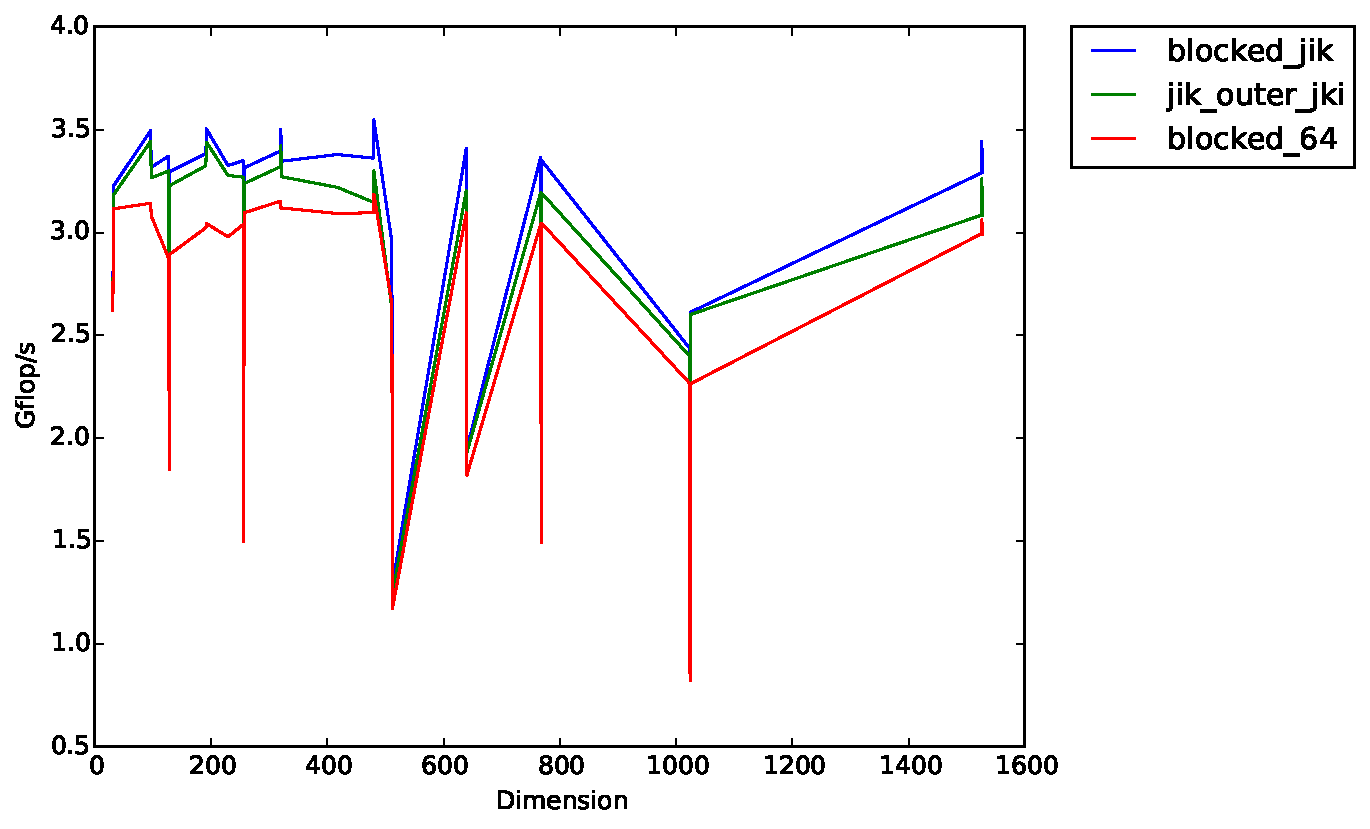
\includegraphics[width=0.9\textwidth]{timing_loop_reorder_fast.pdf}
    \caption{Loop reordering \texttt{ijk} vs \texttt{jik} vs \texttt{jik} and outer loop \texttt{jki}}
    \label{basic_copy_opt}
\end{figure} 

\subsection{Copy Optimization}
\subsubsection{Approach}
In the basic version of dgemm, we see drops near matrix sizes that are a multiple of 2. This is caused by conflict misses due to associative caches. To prevent this, we attempted a copy optimization over the basic dgemm implementation.
\subsubsection{Results}
There is a clear improvement in performance and the conflict misses are converted to gains in performance as seen in Figure \ref{basic_copy_opt}. Copy optimization is clearly a step in the right direction.
\begin{figure}[H]
    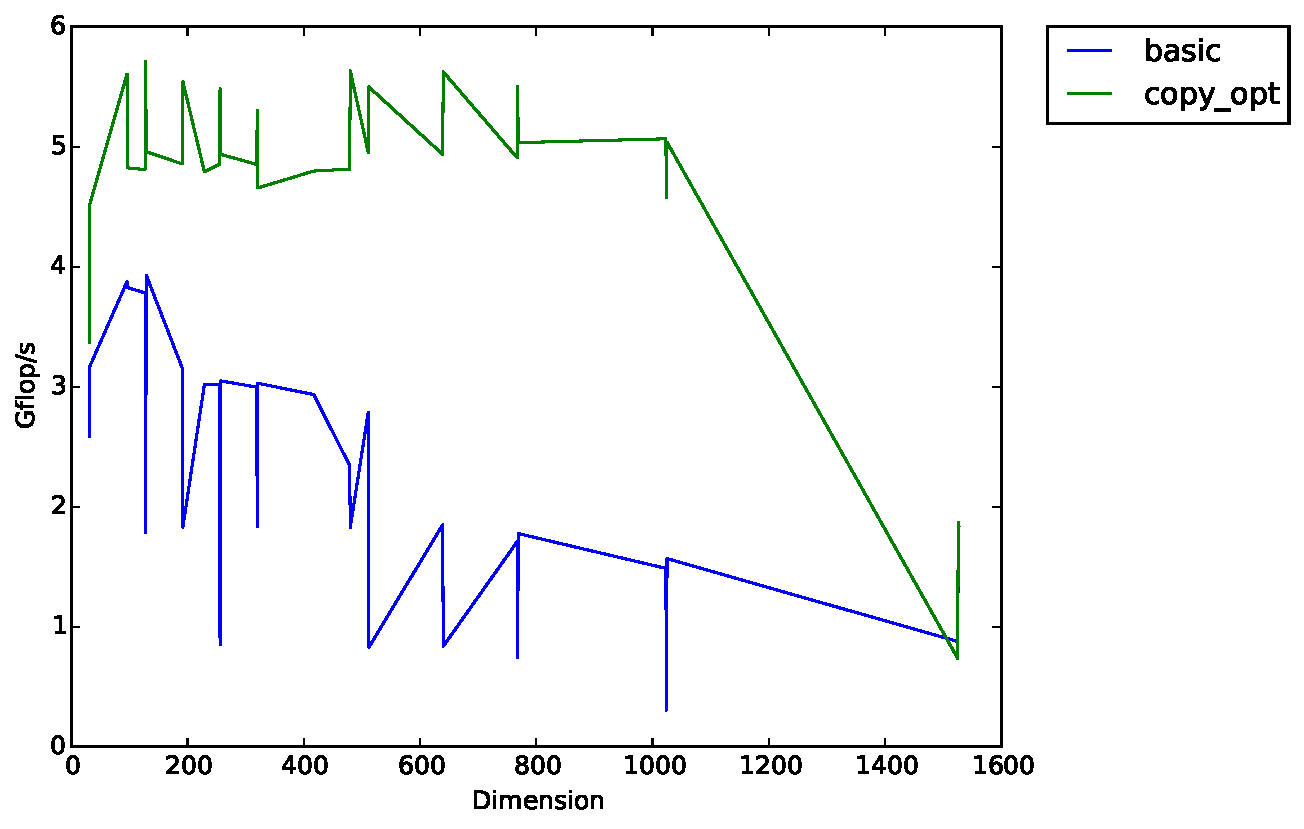
\includegraphics[width=0.9\textwidth]{timing_basic_vs_copy_opt.pdf}
    \caption{Basic DGEMM vs DGEMM with Copy Optimization}
    \label{basic_copy_opt}
\end{figure} 
\subsection{Compiler flags on Copy Optimization}
\subsubsection{Approach}
We use \texttt{-03} and \texttt{-02} optimization flags when we compile the copy optimization code.
\subsubsection{result}
\texttt{-02} optimizer is performing better than \texttt{-03}  especially when the size of the matrix grows larger.
\begin{figure}[H]
    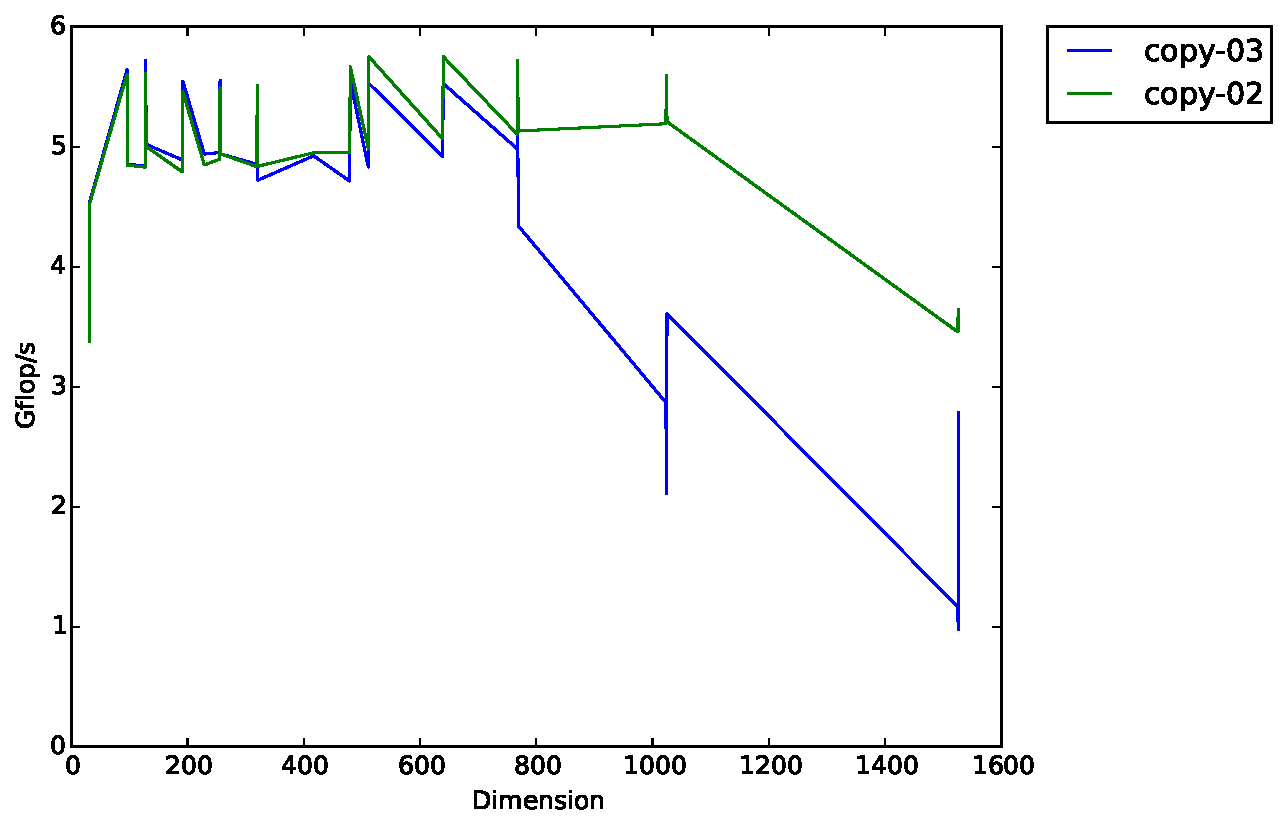
\includegraphics[width=0.9\textwidth]{timing_flag0203_copy.pdf}
    \caption{-03 vx -02 on Copy Optimization}
    \label{0203}
\end{figure}
 

\subsection{Restrict Keyword}

\subsubsection{Approach}
Telling the compiler that our matrix pointers will not be aliasing is another approach suggested on the writeup. 
\subsubsection{Results}

Figure \ref{basic_restrict} shows the performance difference between the basic DGEMM implementation and the DGEMM implementation with the \texttt{restrict keyword}. \texttt{restrict} keyword provides good performance benefits. There is a caveat here since we assumed that the pointer \texttt{A} and \texttt{B} passed to \texttt{square\_dgemm} will not alias. 

\begin{figure}[H]
    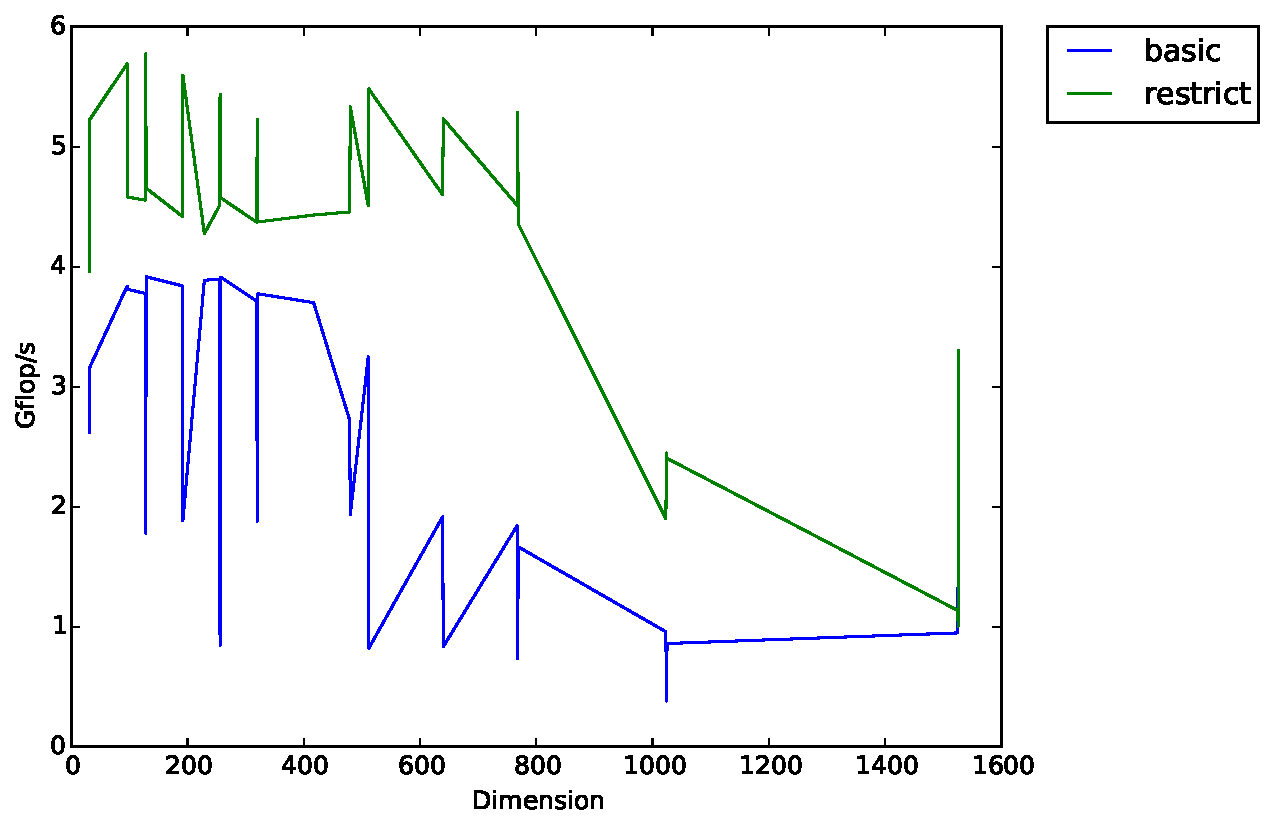
\includegraphics[width=0.9\textwidth]{timing_basic_vs_restrict.pdf}
    \caption{Basic DGEMM vs DGEMM with \texttt{restrict} keyword}
    \label{basic_restrict}
\end{figure} 

To eliminate the aliasing assumption, we intended to couple the \texttt{restrict} keyword and copy optimization to provide a stronger guarantee of not aliasing. The result as shown in figure \ref{restrict_copy_opt} shows that the performance decreases. This may be due to incorrect implementation of the restrict keyword in our code. 

\begin{figure}[H]
    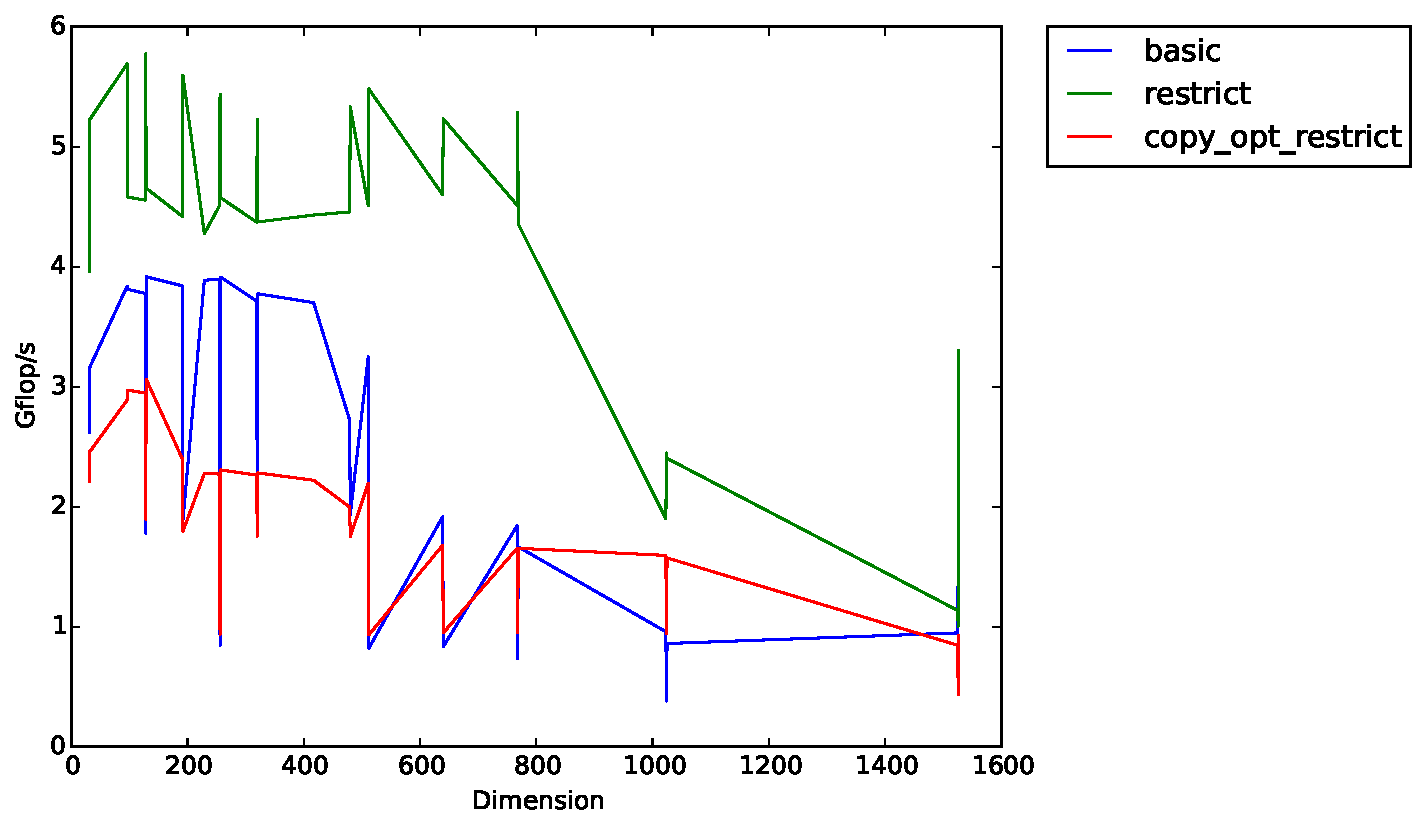
\includegraphics[width=0.9\textwidth]{timing_copy_opt_restrict.pdf}
    \caption{Basic DGEMM vs DGEMM with \texttt{restrict} keyword}
    \label{restrict_copy_opt}
\end{figure} 


\begin{thebibliography}{9}
\bibitem{vectorization} 
Data Alignment to Assist Vectorization. (n.d.). Retrieved September 30, 2015, from \url{https://software.intel.com/en-us/articles/data-alignment-to-assist-vectorization}
 
\bibitem{alignment} 
Memory Management for Optimal Performance on Intel\textsuperscript{\textregistered} Xeon Phi\textsuperscript{\texttrademark} Coprocessor: Alignment and Prefetching. (n.d.). Retrieved September 30, 2015, from \url{https://software.intel.com/en-us/articles/memory-management-for-optimal-performance-on-intel-xeon-phi-coprocessor-alignment-and}

\bibitem{manpages} 
Manpage of ICC. (n.d.). Retrieved September 30, 2015, from \url{http://scv.bu.edu/computation/bladecenter/manpages/icc.html}
 
\bibitem{opt} 
Quick-Reference Guide to Optimization with Intel\textsuperscript{\textregistered} Compilers. (n.d.). Retrieved September 30, 2015, from \url{https://software.intel.com/sites/default/files/compiler_qrg12.pdf}

\bibitem{reports}
Getting the Most out of your Intel\textsuperscript{\textregistered} Compiler with the New Optimization Reports. (n.d.). Retrieved September 30, 2015, from \url{https://software.intel.com/en-us/articles/getting-the-most-out-of-your-intel-compiler-with-the-new-optimization-reports}

\bibitem{ipo}
Improving Performance with Interprocedural Optimization. (n.d.). Retrieved September 30, 2015, from \url{https://software.intel.com/en-us/node/590470}

\bibitem{stepbystep}
Step by Step Performance Optimization with Intel\textsuperscript{\textregistered} C Compiler. (n.d.). Retrieved September 30, 2015, from \url{https://software.intel.com/en-us/articles/step-by-step-optimizing-with-intel-c-compiler}



\end{thebibliography}

 
 
\end{document}
